
%----------------------------------------------------------------------------------------
%	PACKAGES AND DOCUMENT CONFIGURATIONS
%----------------------------------------------------------------------------------------

\documentclass{article}

\usepackage{graphicx} % Required for the inclusion of images
%\usepackage{natbib} % Required to change bibliography style to APA
\usepackage{amsmath} % Required for some math elements 
\usepackage{geometry}
\usepackage{float}
\usepackage{url}
%\usepackage{biblatex}
\usepackage{tocloft}
\usepackage{verbatim}
%\usepackage[toc]{glossaries}
%\usepackage{hyperref}
%\renewcommand{\cftsecleader}{\cftdotfill{\cftdotsep}}

%\makeglossaries

\geometry {a4paper, left = 30mm}
\renewcommand{\baselinestretch}{1.5}
\setlength{\parskip}{1em}
\setlength\parindent{0pt} % Removes all indentation from paragraphs

\renewcommand{\labelenumi}{\alph{enumi}.} % Make numbering in the enumerate environment by letter rather than number (e.g. section 6)

%\usepackage{times} % Uncomment to use the Times New Roman font

%----------------------------------------------------------------------------------------
%	DOCUMENT INFORMATION
%----------------------------------------------------------------------------------------

\title{Giguesaur: iPad Localisation} % Title

\author{Joshua La Pine} % Author name

\date{\today} % Date for the report

\begin{document}

\maketitle % Insert the title, author and date

\begin{center}
\large {Geoff Wyvill and David Eyers}\\
\vspace*{1\baselineskip}
Department of Computer Science \\
Otago University \\

\end{center}
\newpage

\tableofcontents
\newpage

% If you wish to include an abstract, uncomment the lines below
% \begin{abstract}
% Abstract text
% \end{abstract}
%----------------------------------------------------------------------------------------
%	Comments

% Go into detail about working on mac and using xcode and the like due to necessity?

%----------------------------------------------------------------------------------------

\section{Introduction}

% If you have more than one objective, uncomment the below:
%\begin{description}
%\item[First Objective] \hfill \\
%Objective 1 text
%\item[Second Objective] \hfill \\
%Objective 2 text
%\end{description}

\subsection{App Overview}

The aim of the Giguesaur project was to create an iPad application that allows a group of people to collaboratively solve a jigsaw puzzle that is rendered using augmented reality. The virtual jigsaw is assembled on a playing area in the real world. This `game board' is decorated with physical markers which can be tracked using the iPad's camera and the feed from the camera is displayed on the iPad's screen for the user to see. The puzzle's pieces are rendered on the screen in such a way that they appear as though they are in the real world; they look as if superimposed upon the physical game board. The user is able to interact with the puzzle pieces through a user interface on the iPad. Using touch gestures the user can pick up and place pieces down on the board in their desired location. Finally, a large portion of the project was to implement networking so that multiple users are able to collaborate to solve a shared puzzle. %Perhaps reference the augmented reality section. 


\subsection{Motivation}

Our vision for our completed Giguesaur application was allowing a classroom of children, each with their own iPad, to run around and solve a jigsaw puzzle together. Imagine a classroom full of kids where they are all trying to work on a single conventional jigsaw puzzle; such a scheme isn't very practical. The main goal of our project was simply to make a game that is fun for children to play. 


\subsection{Project Format}

Development of the Giguesaur application was a fairly large task, the scope of which was outside the bounds of a fourth year project for a single person. So the project was split up into three separate sections that we combined into the final application. Shahne Rodgers was in control of the networking facet of the project, all of the communication between a device and the server is her domain. Ashley Manson worked on all of the game logic and the user interface, so he developed the game itself, the puzzle piece rendering, and also how the user interacts with the puzzle. I am responsible for the localisation of the iPad, the computer vision element of the project, which I explain in the following section. 


\section{Background}
\subsection{What is Localisation}

Localisation is the task of locating the iPad's camera relative to some real world object. Our application makes use of a physical game board that is tracked with the camera. The current board is a 7$\times$10 checkerboard pattern and using that game board (or tracking marker), we define a real world coordinate system in millimetres. This real world coordinate system is tied to the physical board's position. We use one of the outermost internal corners of the checkerboard as the origin of our real world coordinate system and as we know the dimensions of the squares of the checkerboard we can easily determine the position of other points. \par

Now that we have a real world coordinate system in place we can describe the location of the camera in relation to it (See Figure 1). This position is described by a translation and a rotation vector. These vectors give the camera's translation and change in orientation relative to the origin of our real world coordinate system.\par 

%\vspace*{2\baselineskip}

\begin{figure}[ht]
\begin{center}
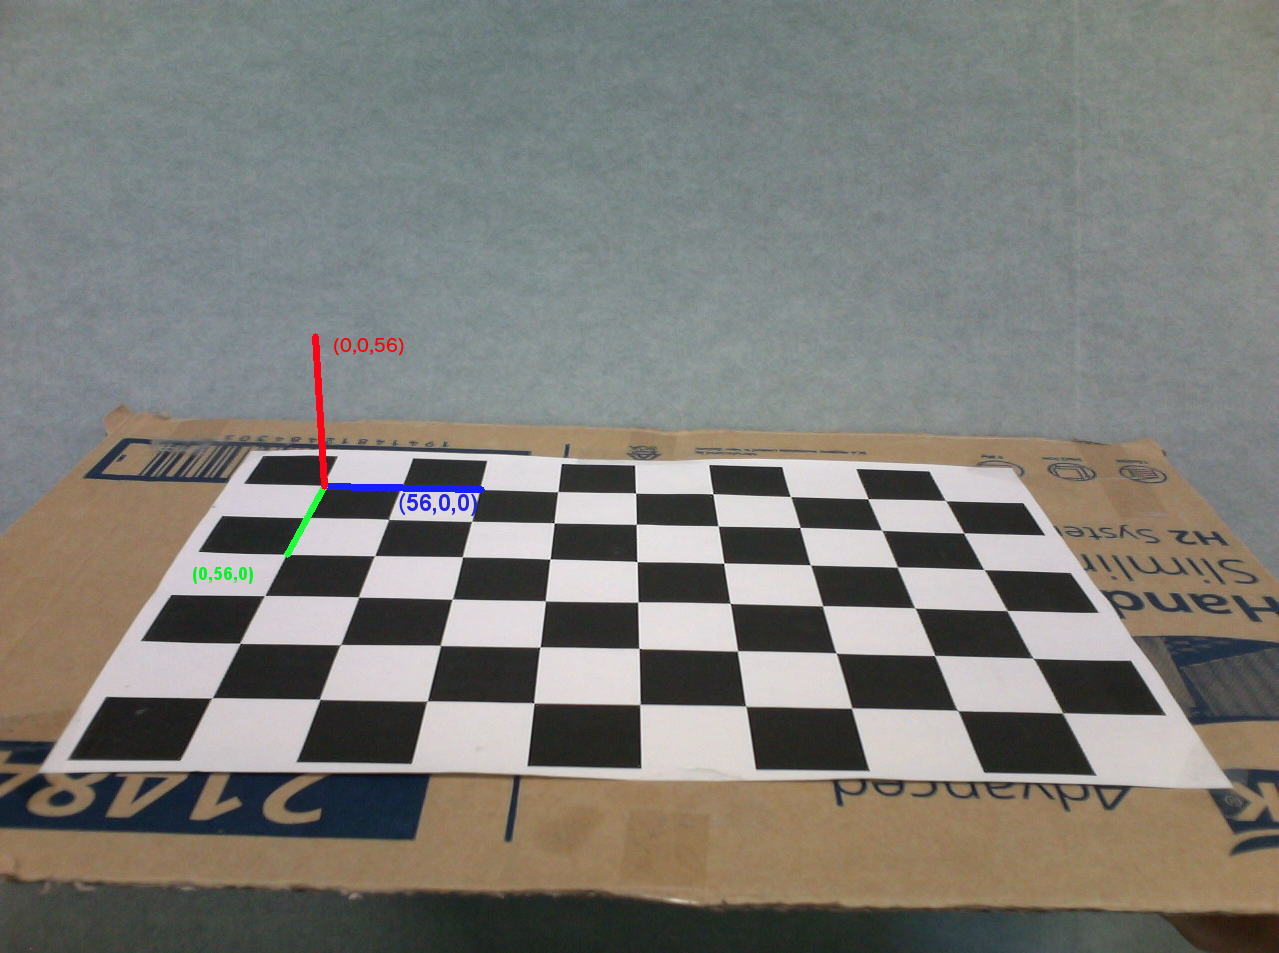
\includegraphics[width=0.65\textwidth]{cam} 
\caption{Real world coordinate system axis markers at the origin.}
\end{center}
\end{figure}

\subsection {Why do we need Localisation?}

Localisation is necessary in order to render our virtual puzzle pieces in such a way that they look as though they lie on the physical game board. 
\vspace*{2\baselineskip}

\begin{figure}[H]
\begin{center}
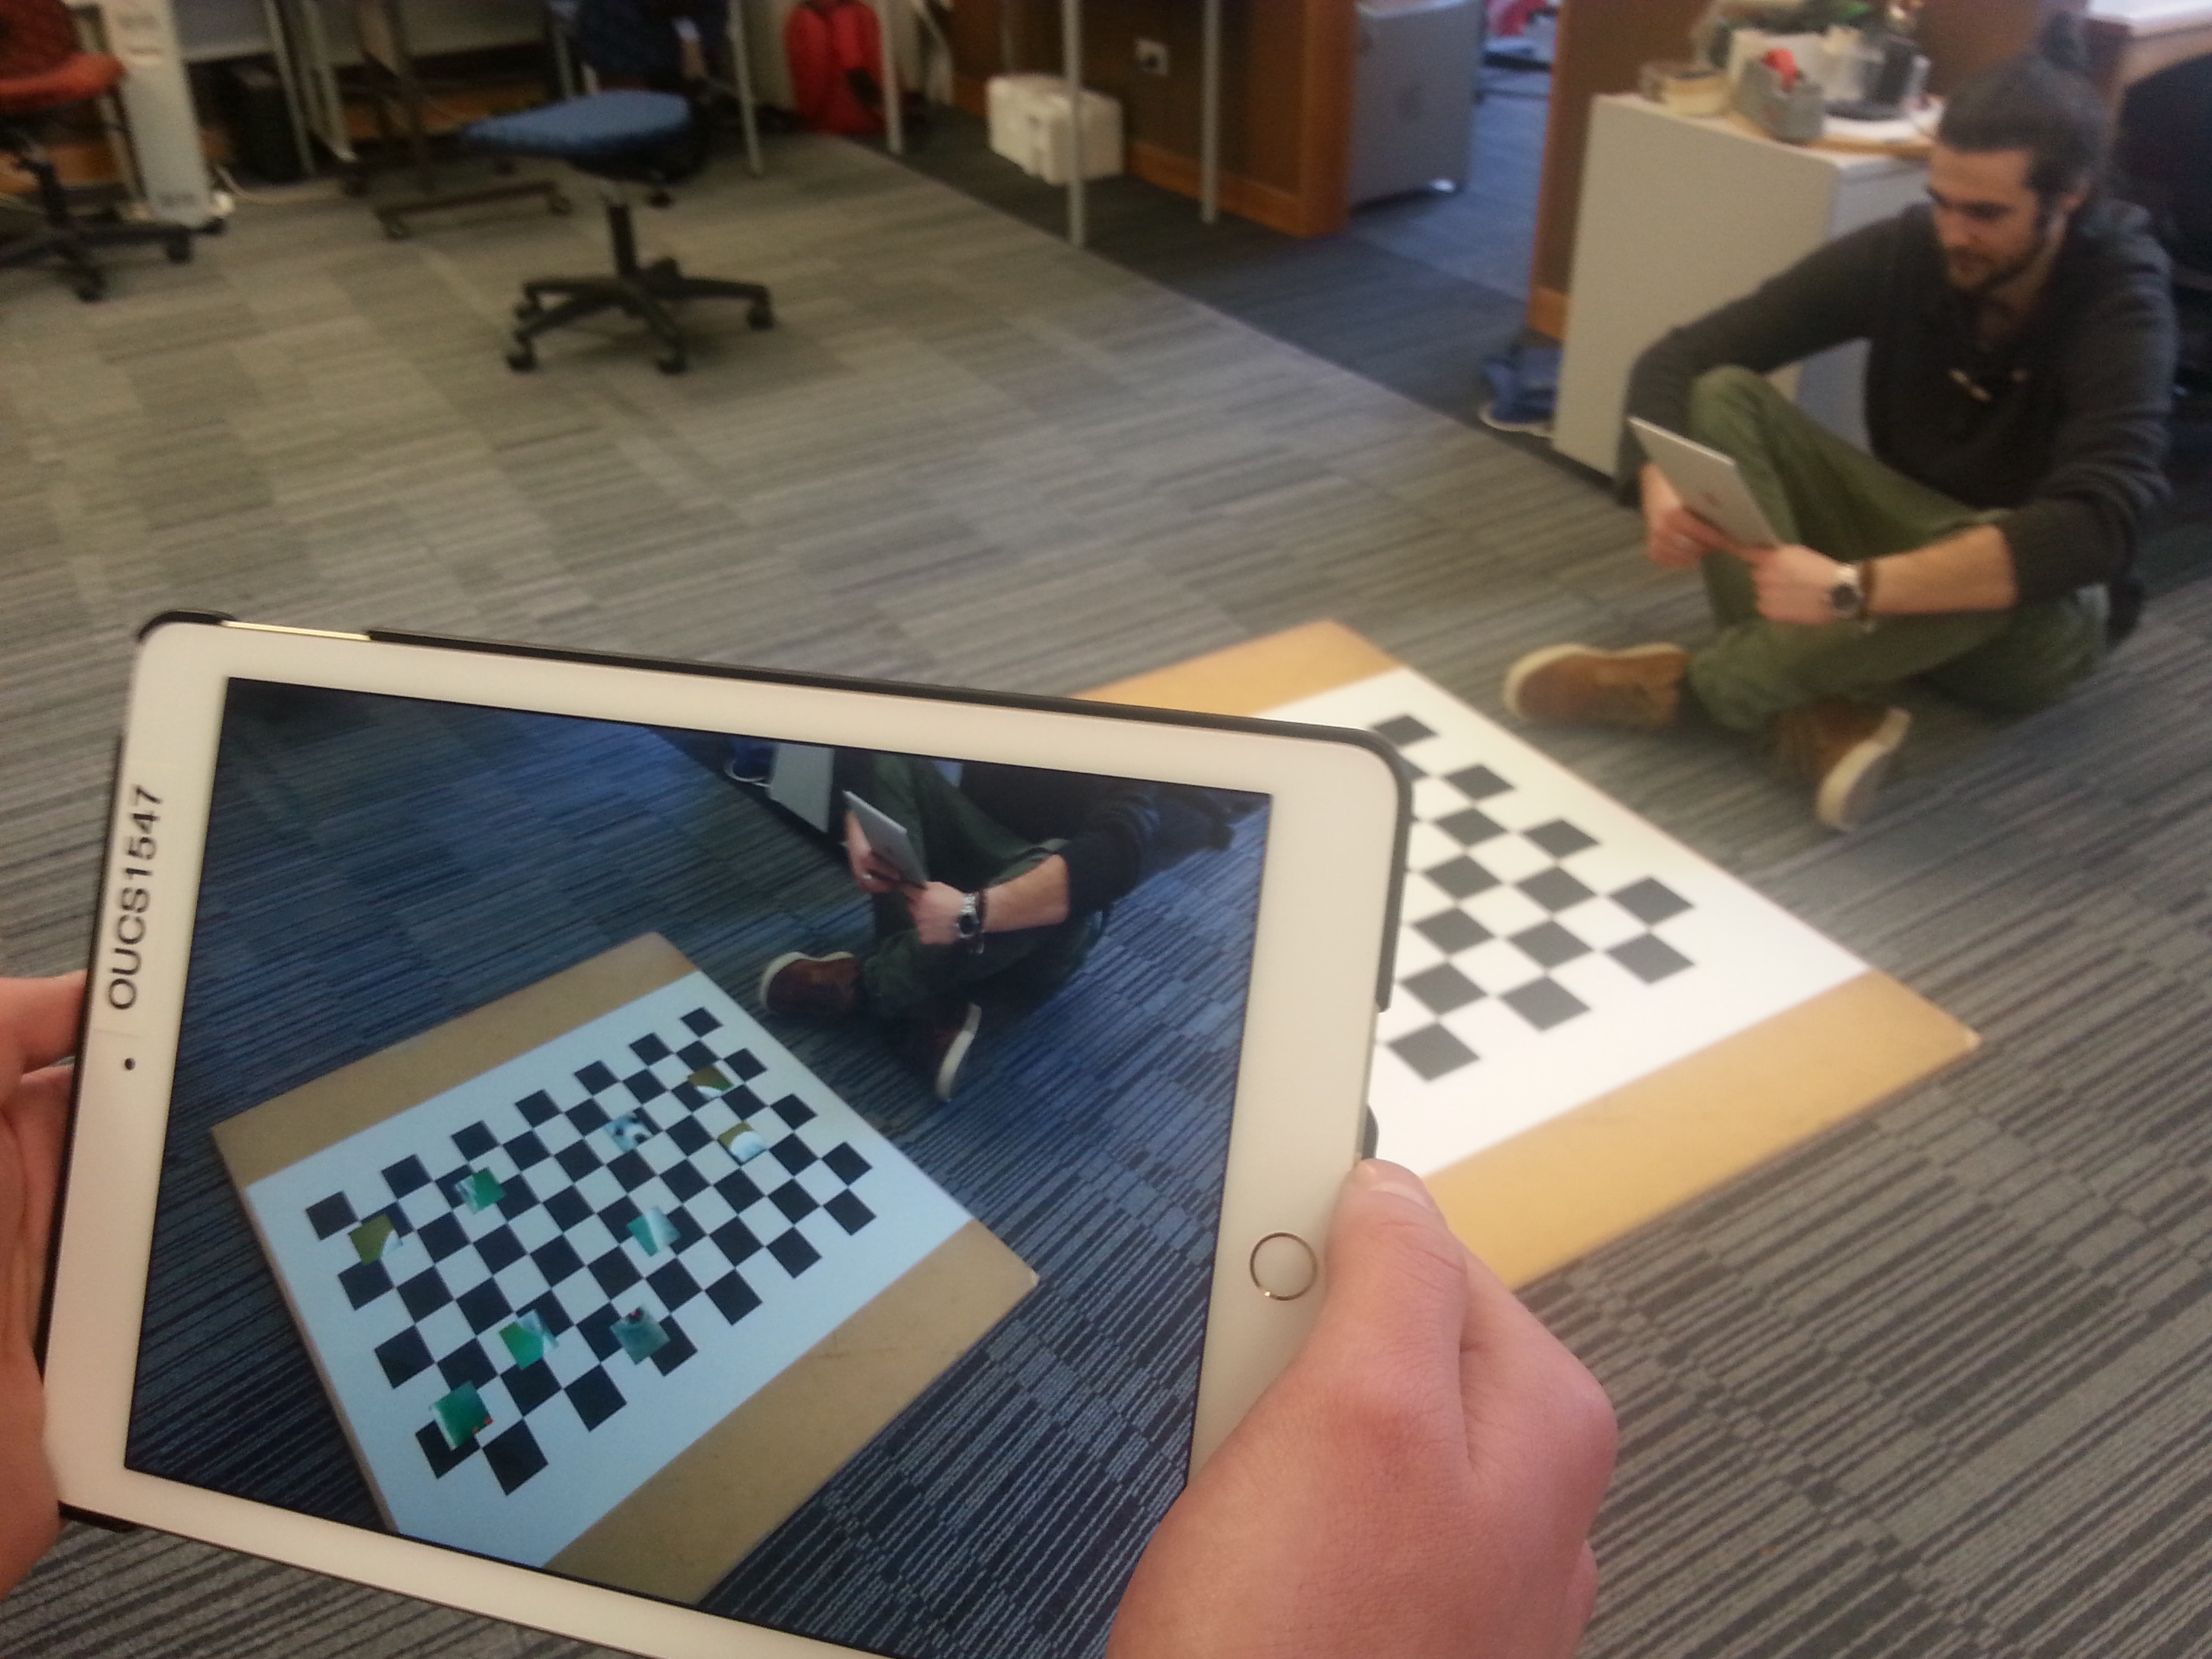
\includegraphics[width=0.65\textwidth]{big_gig} 
\caption{Correctly rendered puzzle pieces.}
\end{center}
\end{figure}

In Figure 2, above, the puzzle pieces have been rendered on the board with the correct perspective. However, if the iPad was in a different place relative to the checkerboard the virtual pieces would have to be rendered differently. It is not difficult to imagine that if the iPad's camera was pointing at the checkerboard from directly above, the pieces would look more or less square. Therefore it is necessary to know where the iPad is in order to render pieces from the appropriate perspective.

\subsection{Augmented Reality}
% Prior work and an overview of other applications and what exactly augmented reality is.
The term `Augmented Reality' refers to the concept of overlaying virtual data on the real world. It is a distinct concept from `Virutal Reality' where the environment that you interact with is entirely digital. Augmented Reality, as the name implies, augments what already exists in the real world. In our case the image that is read from the iPad's camera is augmented with virtual puzzle pieces that you can see through the iPad's display. The localisation, as mentioned in the previous sections, allows us to render the pieces in such a way that the pieces appear to be part of the real world despite only existing digitally. This technique is the essence of an Augmented Reality application and is the reason that my (computer vision) element of the project exists. The reason the Giguesaur application makes use of Augmented Reality is because it is more engaging than a typical puzzle application due to the way the user interacts with it. It is something interesting and different and prior to creating the Giguesaur application nothing quite like it existed. There are iOS jigsaw puzzle apps such as `Jigsaw Puzzle' \cite{ref:JigsawPuzzle} and Augmented Reality iOS games like `ARDefender' \cite{img:ARDefender} but not a combination of the two. 


\subsection{OpenCV}

OpenCV stands for Open Source Computer Vision and it is a software library that is widely used for computer vision tasks. It has functions for easy image I/O, camera initialisation and frame capture, image processing, pose estimation, camera calibration, and iOS support. In short it provided me with most of what I needed to complete my part of the Giguesaur project.

\subsection{iOS vs Android}

% Reference something to make it look more legitimate. 

iOS is the operating system used exclusively on Apple's mobile devices such as iPhones, iPads, and the iPod Touch, while Android is Google's open source operating system for use with mobile devices. The decision to create the Giguesaur application for iOS was made before I undertook the project, however the reasons for that decision are important. 

iOS and Android are the main competitors in the mobile device market, this fact immediately narrows down the choice of operating system. Other mobile operating systems like `Windows Phone' were not considered an option as they are far less popular. One of the core aspects of Android is its `open' nature when compared with iOS, this nature means that Android can be altered to suit any number of different devices. These devices vary in terms of screen size, aspect ratio, and performance, not to mention that Android itself has been through various iterations and each device can run a varying number of these different versions. Conversely iOS is a closed operating system, you can't freely modify iOS to run on different devices and as a result the total number of devices and the variation between each of these devices is small when compared to Android. 

When developing a mobile application these differences between the operating systems is one of your main considerations. For a three person team, the level of variation present among devices is far too much. What might work well on one device and version of Android might break on a different device or operating system version. The argument could be made for supporting a small subset of android devices but even then the lack of standards between each would be too much to deal with. iOS in comparison has only a few devices and operating system versions that need support and most of the time there are no differences to handle between each of these. 

We designed Giguesaur to be playable by a class-room sized group of kids. In order to support that goal the application needs to be run on a decent number of devices. As people are likely to have iOS devices already, and with all of the above in mind, creating the Gigusaur application for iOS, rather than Android, was the only sensible choice. 

\subsection{Apple and Xcode}

Working with iOS requires the use of Mac OSX and therefore the use of Apple computers. 

Xcode is the name of Apple's integrated development environment and it is essential when developing for the iOS platform because Apple requires that you use Xcode to upload code to an iOS device.

\section{Achievements}

\subsection{Overview}

My work on the Giguesaur project began by researching marker tracking as it was described in the project specification. I came across a variety of articles on the subject but of particular interest was the paper behind the ARToolkit \cite{artoolkit}, which is a widely used marker tracking package. I then began to use OpenCV as I would need image processing capabilites and followed that by learning about pose estimation and camera calibration, which are large components of my project. After implementing these processes I began to port my code to the iOS platform. Once the porting to the iOS platform was complete the task became integration, which brought with it an new set of challenges. 

%More detail here, Perhaps need to go into fine detail about how the pose estimation algorithm works. Perhaps start by describing what it does, finds a correspondence between real world and image-space coordinates. 
\subsection{Pose Estimation}

Pose estimation is the name of the process which is used to locate a camera. It is the core process for my part of the Giguesaur project. Specifically such an algorithm uses the co-ordinates of points in the real world and the co-ordinates of the corresponding points in the image to define a relationship between these two systems. The idea is that once you have calculated the relationship between these two systems you can then find a real-world point's image-space location. This is necessary as the puzzle pieces' locations are defined in terms of our world-space co-ordinate system but are, of course, displayed on the iPad's screen. 

%Talk about homography here?
%The relationship between these two systems is called a 'homography', which is the name given to the mapping from one plane to another. 

A pose estimation algorithm has a number of requirements before its output can be calculated. \par

The first thing required is that the camera you are locating must be calibrated. The camera calibration process is described in Section 3.3. \par

Secondly the algorithm requires the coordinates of a set of points in world-space. In our case this set contains all the internal corners of our checkerboard pattern. As the origin of our world-space coordinate system is one of the outermost internal corners and we know the side length of the squares we can then set up a nested for loop block where each loop increments by the square side length. Each iteration pushes a 2D vector comprising an $x$ and $y$ coordinate to an array. Note that the $z$ coordinate can be excluded because our checkerboard is flat and so all the points are at $z = 0$. Once the nested for loop block has finished executing we have an array containing the coordinates of all the chessboard's internal corners. \par

The last requirement for a pose estimation algorithm is a way to find the points in image-space that correspond to these points in world-space. As the checkerboard image is a common pattern used in camera calibration routines OpenCV has a built in function called findChessboardCorners. This function locates the internal corners of a chessboard and outputs an array of their coordinates in image-space. \par

Once all of the above has been calculated then a pose estimation algorithm can be run with the arrays of points as input along with matrices related to camera calibration. The algorithm I use in this project is a OpenCV function called SolvePnP \cite{calib3}. Writing my own routine for such a task would be quite an undertaking and it is only one part of my piece of the project. The SolvePnP function then outputs two vectors, one for rotation and one for translation. These vectors together describe the location of the camera relative to the checkerboard. \par

The rotation and translation vectors can be used to transform points in world-space to points in image-space. So we can take points defined in world-space and transform them using these vectors in order to render them in the correct position in image-space. OpenCV provides a function that projects points in world-space to points in image-space. This function takes the vectors as input along with a set of world-space coordinates and returns an array of image-space coordinates. I have used this function to superimpose a wire frame cube onto the checkerboard, which you can see below in Figure 3.


\begin{figure}[H]
\begin{center}
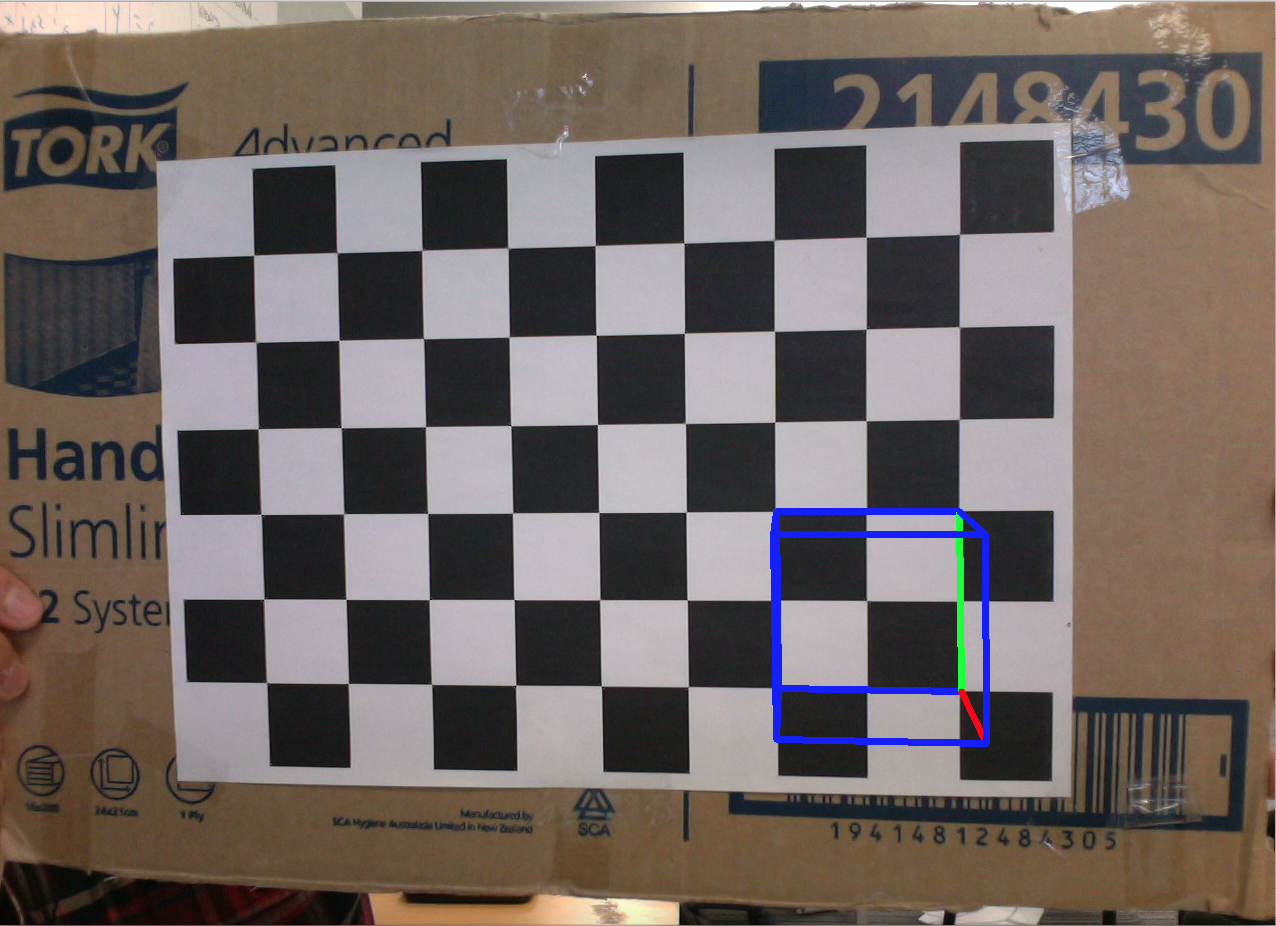
\includegraphics[width=0.65\textwidth]{arCube} 
\caption{Augmented Reality wireframe cube.}
\end{center}
\end{figure}

\subsection{Camera Calibration}

Camera calibration is a necessary step in the process of pose estimation. Figure 4, below, is a simplified diagram of an ideal pinhole camera model. A pinhole camera takes an image of the real world and projects it onto an image plane \cite{pinhole} as seen in the image below. In reality a pinhole does not receive enough light in order to do this, so a lens must be used to focus enough light to project the image. Using a lens introduces a source of several forms of distortion \cite{calib1}. This distortion must be accounted for when performing image processing tasks such as pose estimation. \par

The characteristics of the camera must also be determined. These characteristics include the pixel coordinates of the principal point and the scale factors of the x and y image-space axes. The principal point is where the optical axis of the camera intersects the image plane \cite{wikicalib}.

\vspace*{2\baselineskip}

\begin{figure}[H]
\begin{center}
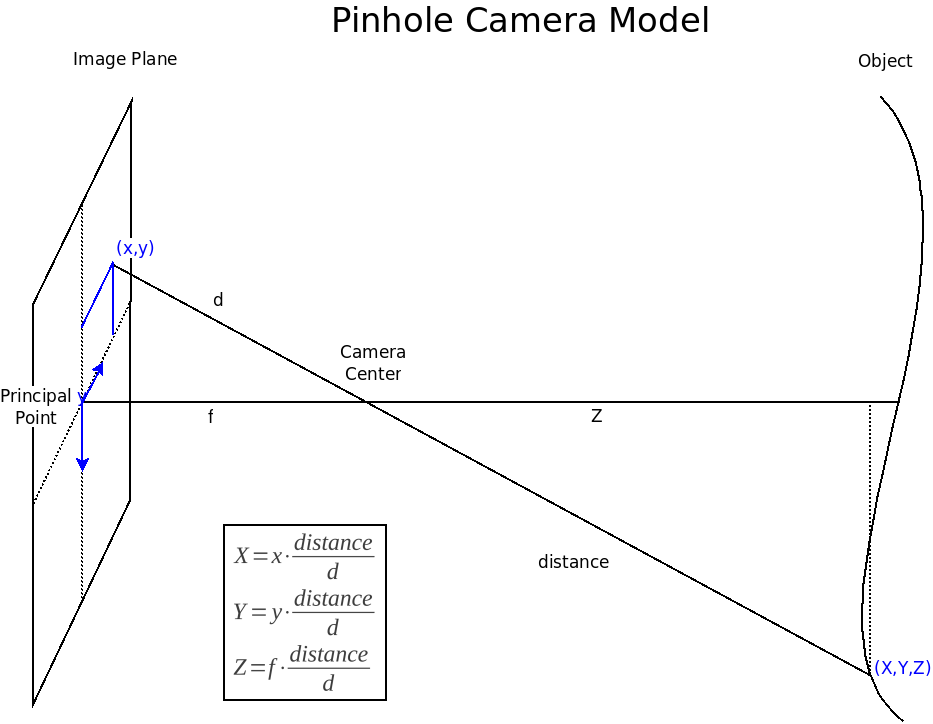
\includegraphics[width=0.65\textwidth]{PinholeCameraModel}
\caption{Source: http://docs.mitk.org/nightly-qt4/PinholeCameraModel.png}
\end{center}
\end{figure}

Together these camera characteristics and distortion measurements are known as the camera's intrinsic parameters. These parameters are required when calculating the rotation and translation vectors that describe the camera's location, otherwise known as the camera's extrinsic parameters. \par

I use OpenCV for my camera calibration routine which is based on the calibration technique developed by Zhang \cite{zhang}. I start by taking a number of photos, from different angles, of a calibration pattern \cite{calib2}. Camera calibration routines make use of a few common patterns with easily detectable features, one such pattern is a checkerboard. So in our case the checkerboard is both the game board / tracking marker and calibration pattern. The ideal number of photos is around 15--20, a value I found by experimenting. Fewer than 15 and the pose estimation begins to become erratic, resulting in distorted augmented reality models. I then create a list of those images in XML format with a small program found on the OpenCV Github page \cite{opencvGit}. Once the image list has been generated and the parameters of the calibration defined in a separate XML file I run the full calibration program provided on the OpenCV Github. The result of this calibration procedure is an XML file containing a “Camera Matrix”, which is a 3$\times$3 matrix describing the camera's characteristics as mentioned above, and a “Distortion Coefficients” matrix, which is a 5$\times$1 matrix describing measures of various forms of distortion. These matrices are parsed by my program to be used by the pose estimation function. 

The camera's characteristics and distortion must be modelled  because an image from a camera does not accurately represent the real world. The characteristics of the camera, as mentioned above, and the various forms of distortion introduced by the use of the lens cause an image produced by the camera to be distorted in various ways. For example, straight lines in the real world do not appear straight in the captured image. So using the calculated characteristics and distortion measures when performing image processing allows you to account for these inaccuracies.


\subsection{Porting to iOS}

Making our application compatible with iOS was a significant portion of the project. Once I had an augmented reality prototype working correctly on an iMac I began to port my existing code over to the iOS platform. \par

Developing for iOS is different from developing for a regular computer. Code that works on a regular iMac will not work on an iOS device without modification and the use of different APIs is usually required. As my code makes heavy use of OpenCV functions I had to use the OpenCV framework for iOS, and this proved to be a more complicated exercise than I had anticipated. \par

For example, retrieving a frame from the camera on the iMac requires very little code to achieve. It is simply a matter of declaring a VideoCapture object and a matrix to store the pixel values and then the use of a single command to load from that VideoCapture object into that matrix. In iOS the same process requires a number of initialisation steps in order to begin using the camera. This includes things like setting the video stream quality, orientation, and which camera to use. \par

\subsubsection{Camera Setup and Calibration}

I began my work with iOS by attempting to retrieve a frame from the iPad's camera. The first thing I tried was using the CVVideoCamera library that comes packaged with the OpenCV framework for iOS. I was able to get a frame from the camera and process it before displaying it on the iPad's screen without much difficulty. However when I attempted to complete more complex tasks problems began to appear. \par

The iPad's camera, unlike my iMac's built in camera, has an auto-focussing lens. When a scene is viewed the lens automatically adjusts to bring the scene into the sharpest focus possible. This turned out to be a large problem as the intrinsic parameters of the camera are only useful for a given focus setting and all of the calibration images must be taken at the same focus setting. As the lens was automatically focussing when I took the calibration images the process was flawed even at that stage. \par

In order to overcome this problem, more information was required. I needed to be able to get and set some value that represents the lens position \cite{xamarin} then hopefully I could take an adequate set of calibration images and calculate the camera's intrinsic parameters for that value. My initial plan was to calculate the camera's intrinsic parameters for a variety of focus settings and, when the app is operating, measure the focus setting and then set it to the nearest value with stored intrinsic parameters. This need for more information led to the use of Apple's AVFoundation framework \cite{apple_class}, which is a more complex but flexible framework for using the iPad's camera. 

I swapped the video framework I was using from OpenCV's CVVideoCamera to Apple's AVFoundation. Initially this was not a particularly painful process with AVFoundation requiring slightly more code to initialise but giving more freedom in return. After initialising a number of various video input and output objects of Apple's design I was ready to test my plan for calibration. 

I succeeded in using the framework to perform an experiment on several focal settings, the focal setting being a number in the range 0--1. Firstly I created an application and tied a slider to the focal setting, so when I moved the slider to the right the focal setting would increase. This application gave me an insight into how the iPad's camera feed looked at different focal settings. With this information I wrote a small program that would take a picture at a focal setting when the iPad's screen is pressed and then increment the focal setting by 0.1, this increment would take place only twice before the focal setting was reset to the original value. The initial value for the focal setting was chosen to be 0.7. The reason for this seemingly arbitrary value is that when the camera was set to 0.7 the image from the camera looks fairly in focus in all cases except for when the camera is very close to some real world object. The reason for the focal increment only occuring twice before reset is that I only wanted a small set of data to consider and then based on my findings I could gather more data if necessary. \par

Using this program I took 3 pictures, one for each focal setting 0.7-0.9, of 20 different views of the checkerboard. I then fed each of these sets of images into the camera calibration routine to calculate the camera matrix and distortion coefficients matrix for each focal setting. I was hoping that I could identify some simple relationship between the focal setting and the camera and distortion coefficients matrices based on the data I had collected. While each of the camera matrices was the same at each focal setting the distortion coefficients matrix was different and I was unable to model these differences. I then thought about following through with the plan I discussed above by calculating matrices for a variety of setttings and changing between them depending on the measured focal value. However this soon turned out to be more trouble than it was worth and I decided on a fixed focal setting of 0.7 which looks reasonably focussed at most distances.


\subsubsection{Image Handling}

One of the major difficulties in using the AVFoundation framework comes in processing an image and then displaying it to the screen. Displaying the video feed to the iPad's screen is trivial and is done via what Apple calls a `Preview Layer'. If you wish to process a frame and then display it the task becomes much more difficult. When utilising the `Preview Layer' the video feed gets displayed directly to the iPad's screen and each frame is stored in a buffer for processing that is separate from the main thread of execution. %That is accessible only from a separate thread of execution?
 Any attempt I made to remove the `Preview Layer' and set the current view to the last frame received resulted in the camera feed closing. 
%Might not be needed man.
 I was still working on this problem when the decision was made to start integrating each part of the project into one application.

Another problem with the AVFoundation framework is that the buffer where incoming camera frames are stored is of a particular type called a `CMSampleBuffer'. There was no simple conversion from the sample buffer to an OpenCV Matrix, which I required in order to utilise the various OpenCV functions. On investigation, I discovered that Apple's frameworks provide functions that return various pieces of information about the size and format of a given buffer. Using some source code I found that performed a similar function \cite{iOS} %source needed here
I managed to convert the `CMSampleBuffer' to an OpenCV Matrix upon which I could utilise OpenCV functions for processing the image.


\subsection{Integration}

After a semester of work on each of our individual portions of the project the decision was made to begin integrating the components into a single application. Integration is a difficult task and had we continued working on our components separately we might never have produced an application that could be considered to work correctly.

The first task for integration was to set up a joint Xcode project that we could all work on that was backed up with version control. When creating an Xcode project you have to be sure to link all of the libraries you are going to use so that your code will compile correctly. iOS makes this step easy as each library has a framework object that you can include in your project from the menus in Xcode. Once we had a blank project set up we copied all of our source code into it and began the task of integrating each component into a single working application. Doing this required us to link the relevant parts of each source file together using import statements and references and replacing dummy method calls. Much earlier in the project Ash, Shahne, and I made a rough plan about which components should interact and how they would do so, however when it came time to put this plan into practice it didn't go smoothly. 

When considering how to structure a program that you haven't fully figured out yet you have to make assumptions. The problem is that you don't know the best way until you have tried to implement something and that is what we found when we began integration. So a large part of the difficulty of integration is accounting for assumptions made or things not considered during the design process. As we were working on something new to us there were a few such instances. These instances include things like different ways of representing the same data, type incompatibilities and so on. Another aspect contributing to the issue of integration is that as each of us researched and discovered things about our parts of the project our ideas on how to implement things changed.

Once we had integrated the code into a compilable project we could continue working on completing the application. From this point on much of the work I did was in direct collaboration with Ashley Manson who worked on the Game Logic and Interface. 

\subsubsection{Displaying Camera Frames}

Displaying a processed camera frame to the screen was a non-trivial problem that was put to one side while we built our joint project. Ashley's game logic and interface had progressed to the point of having a working jigsaw puzzle that was rendered with OpenGL and displayed to the screen, with pieces that could be moved using touch gestures. So the next step was to combine Ashley's game and interface with my computer vision component and this meant having the video feed as a background. 

Ashley had a method for displaying a background image on the screen upon which to render the puzzle pieces, so we reasoned that we could pass the frame from the camera to the background image rendering code and this would result in the video feed being displayed to the screen. This involved a few image format conversions as well as an extra method.

Each frame from the iPad's camera is stored in a CMSampleBuffer and a method operating in a separate thread is executed whenever that buffer is written to. Within that method the image is converted to an OpenCV matrix so that the pose estimation function could give us the rotation and translation vectors required to render the puzzle pieces in the correct perspective. %Might be worth taking out the mention o pose estimation here, talk about it later anyway.
After that the image is converted to a UIImage for compatibility with Ashley's code and an auxiliary method in the game logic code was called and sent the UIImage. This auxiliary method is necessary as the buffer method operates in a separate thread and a method call must be performed on the main thread in order to send it data. The auxiliary method then calls the background render method and passes it the image for the background. %Dunno about this next part. come back to it.
Unfortunately this broke the puzzle piece texture rendering which Ashley had implemented, but we decided to put that aside in order to work on rendering the puzzle pieces in the correct perspective.

We made an earlier attempt at rendering the processed camera frames to the screen using the `Preview Layer'. We reasoned that we should be able to render the puzzle pieces on a separate layer using OpenGL and then render that layer on top of the `Preview Layer'. From our reading we discovered that this is possible \cite{preview}, however, we could not get it to work. Either we could display the pieces with a block colour background or we could have the video feed but not both at the same time. After struggling with this approach we decided to try using Ashley's background image method.

\subsubsection{Perspective Rendering}

I had previously used OpenCV in order to render simple geometry in perspective as a means of testing the pose estimation function. To do this, world-space coordinates must be transformed into image-space coordinates before being drawn on the background image. OpenCV provides such a function that accepts the previously calculated rotation and translation vectors as arguments along with a vector of world-space coordinates and returns the corresponding image-space coordinates. As our pieces are stored in world-space we reasoned that we might be able to use this function to render pieces in the correct perspective as simple quads. 

When exploring this option further we discovered that OpenCV has a function for calculating a perspective transformation between four pairs of vertices \cite{cv_render}. This effectively returns a matrix that describes the transformation from one quad to another. You can use the OpenCV function warpPerspective to apply that transformation to a given image. So rather than render quads for the pieces and texturing them we decided to try transforming the textures directly and superimposing them on the background image in the correct position. 

Our implementation of this works piece by piece and begins by creating 4 3-vectors that represent each vertex of the piece. These are the world-space coordinates of the corners of each piece. Then we calculate the image-space coordinates for each of the vertices so we know where on the screen to render the image. We then create a sub-image from the image used to texture the puzzle, this sub-image is the piece of the texture image that represents the piece. Following that we calculate the perspective transformation from the sub-image to the image-space coordinates for the piece. This operation basically maps a small piece of the full puzzle image to where the piece should be displayed on the board. After applying the perspective transformation to the sub-image we are left with an image that is the same size as our background image but all of it is empty space besides the pixels that make up the sub-image. We then superimpose this image onto the background and repeat for each piece. This whole operation is done every frame. 

Prior to this implementation we attempted to initialise the OpenGL camera to render the pieces in the correct perspective using the results of the pose estimation algorithm. This required several matrix multiplications and a transposition, as well as an auxiliary method for calling from a separate thread. This approach resulted in the pieces disappearing from view. We attemped to debug our method but after progress on the application stalled for too long we decided to use OpenCV for the prespective rendering. 

\section{Results}

The application works as shown in our accompanying video (see Appendix). When the application is started and the iPad's camera is pointed at the checkerboard pattern the user is presented a view of the world obtained from the iPad's camera. The puzzle pieces are rendered on top of that view in the correct perspective, and by tapping a piece and then a place on the screen, the user can pick up and place the piece in a desired position. When a piece is placed close enough to a correct neighbour in the puzzle, the two pieces will snap together. The puzzle is considered solved when all the pieces have `snapped' to their correct neighbours. Players are able to work together to solve the puzzle. 

In particular, the localisation works correctly although it is not yet fast enough to be practical. Currently the application runs at around five frames per second. Below, in Figure 5, are pictures of Giguesaur running. The image on the left shows the puzzle and game board from a high angle, while the image on the right shows a low angle view. This serves to show how the puzzle pieces are rendered depending on the iPad's position in relation to the checkerboard pattern. 


\begin{figure}[H]
\begin{center}
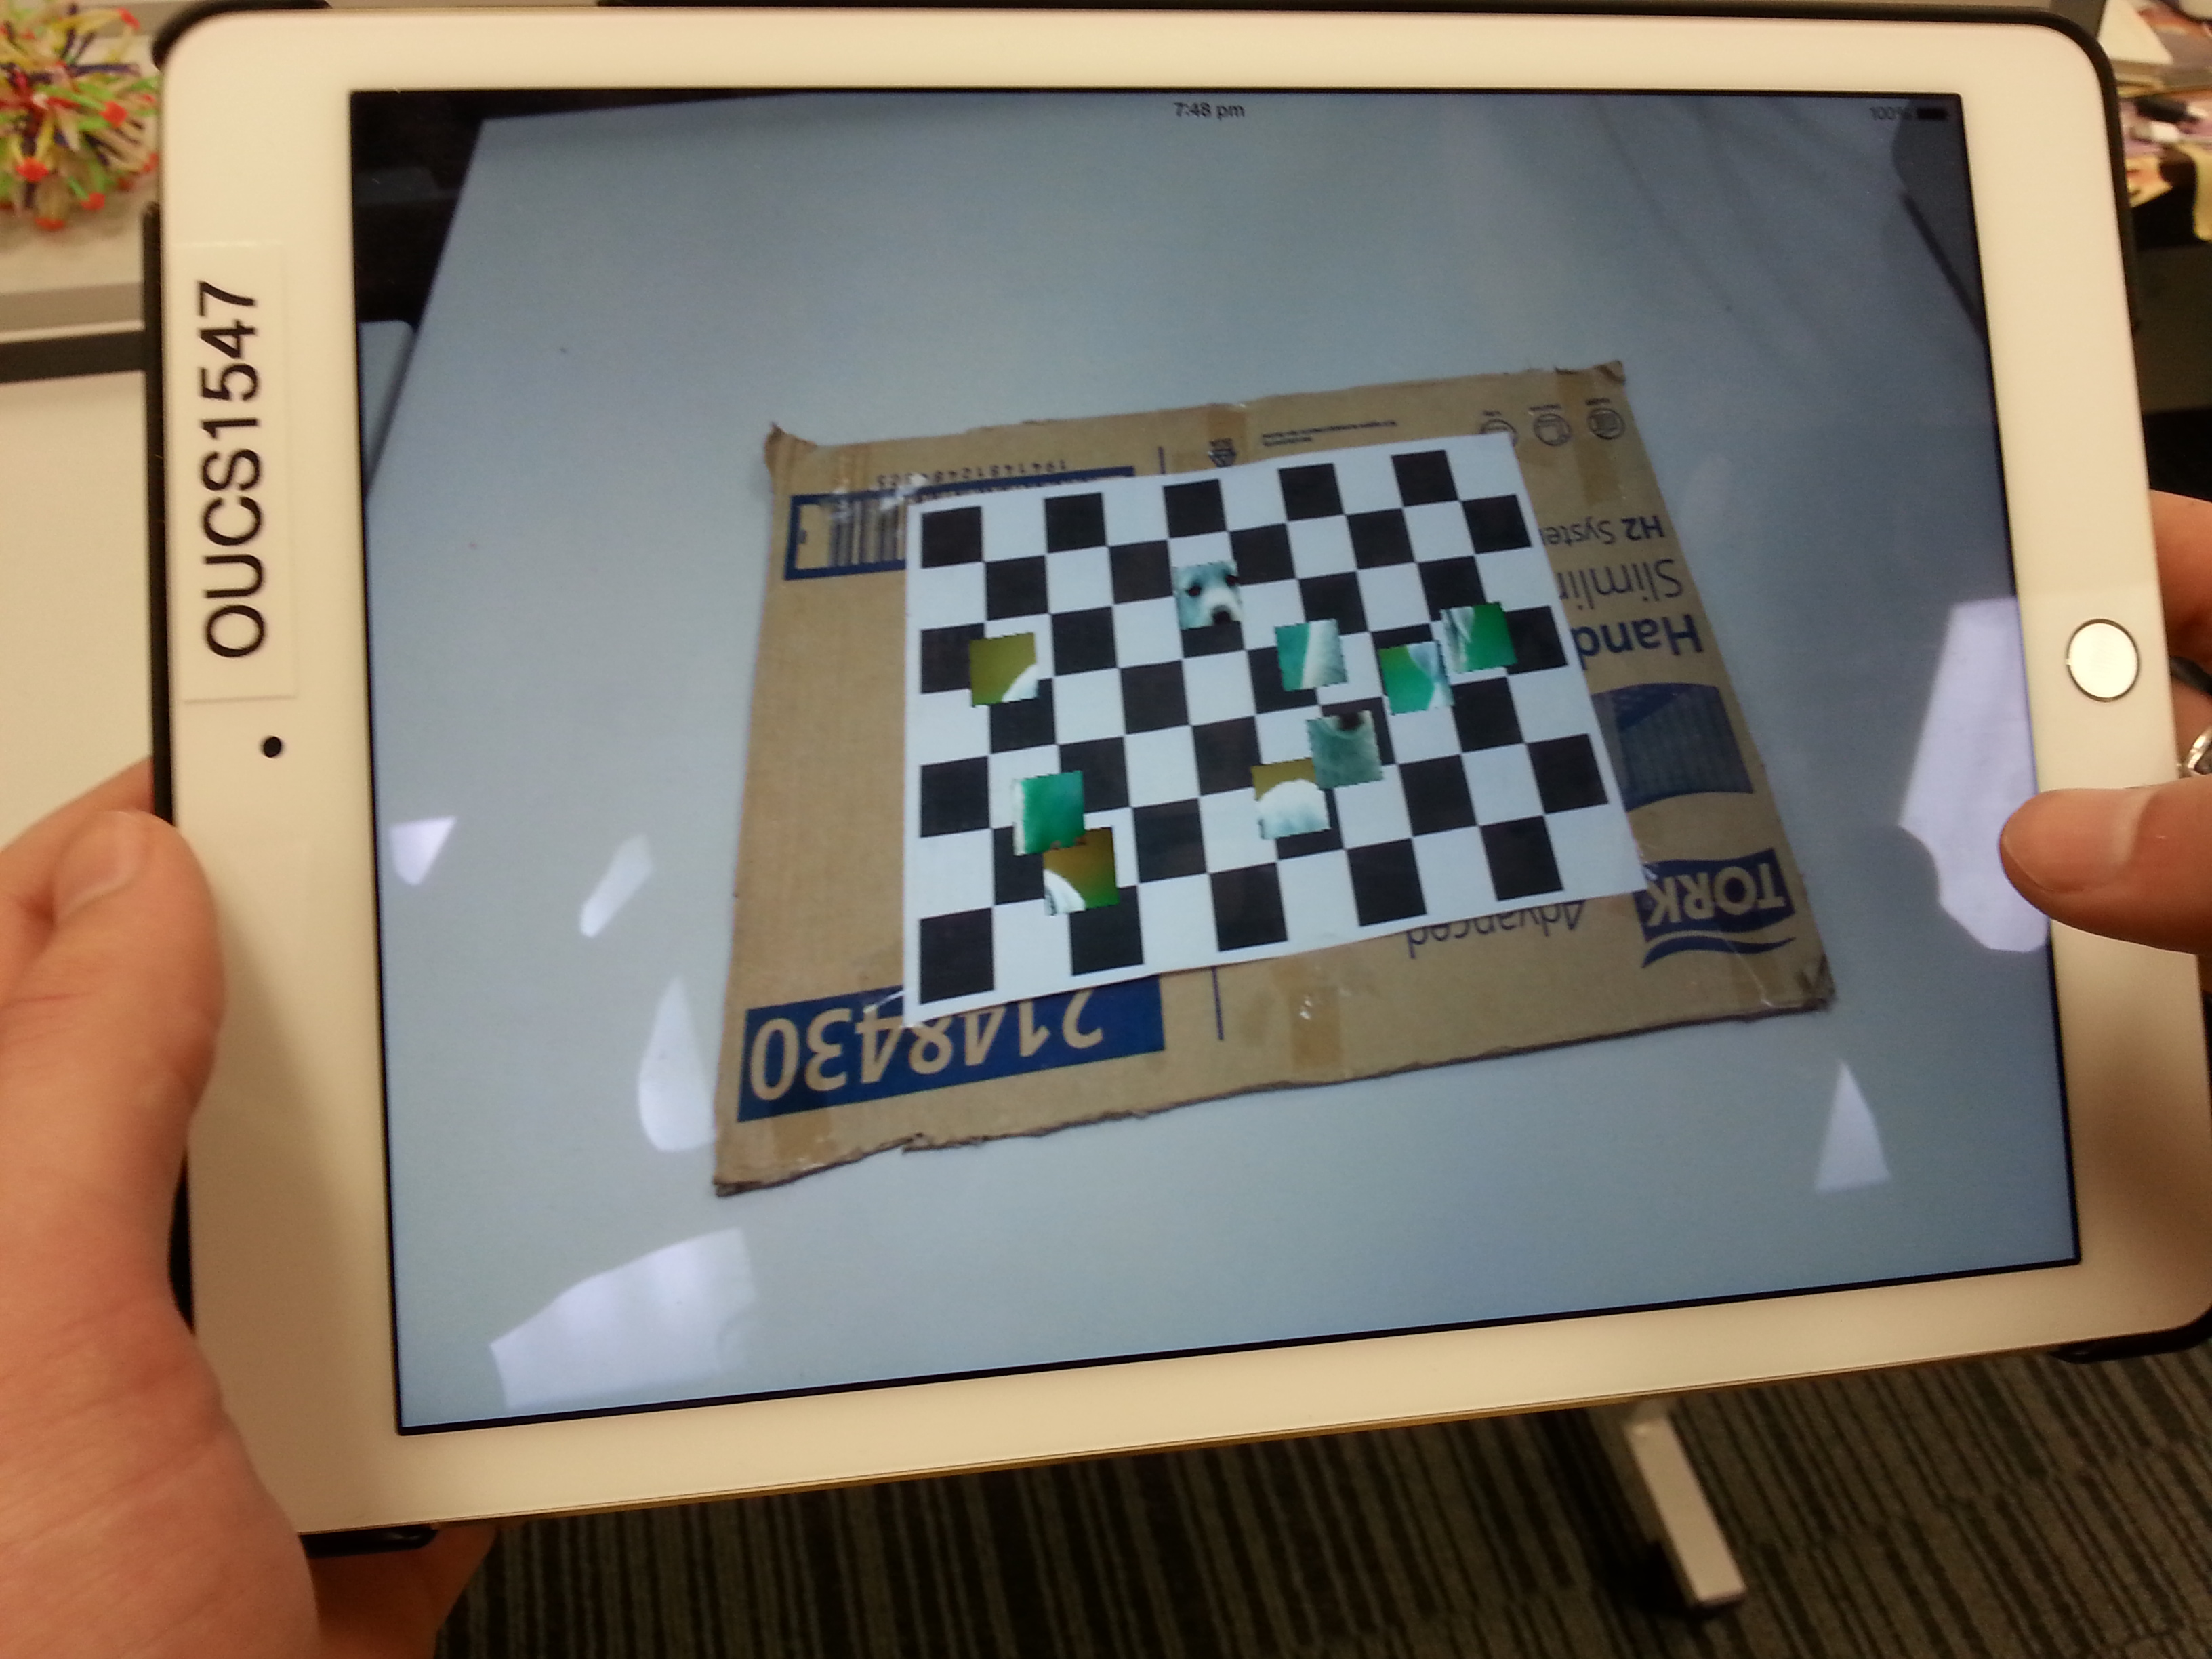
\includegraphics[width=0.49\textwidth]{high_angle}
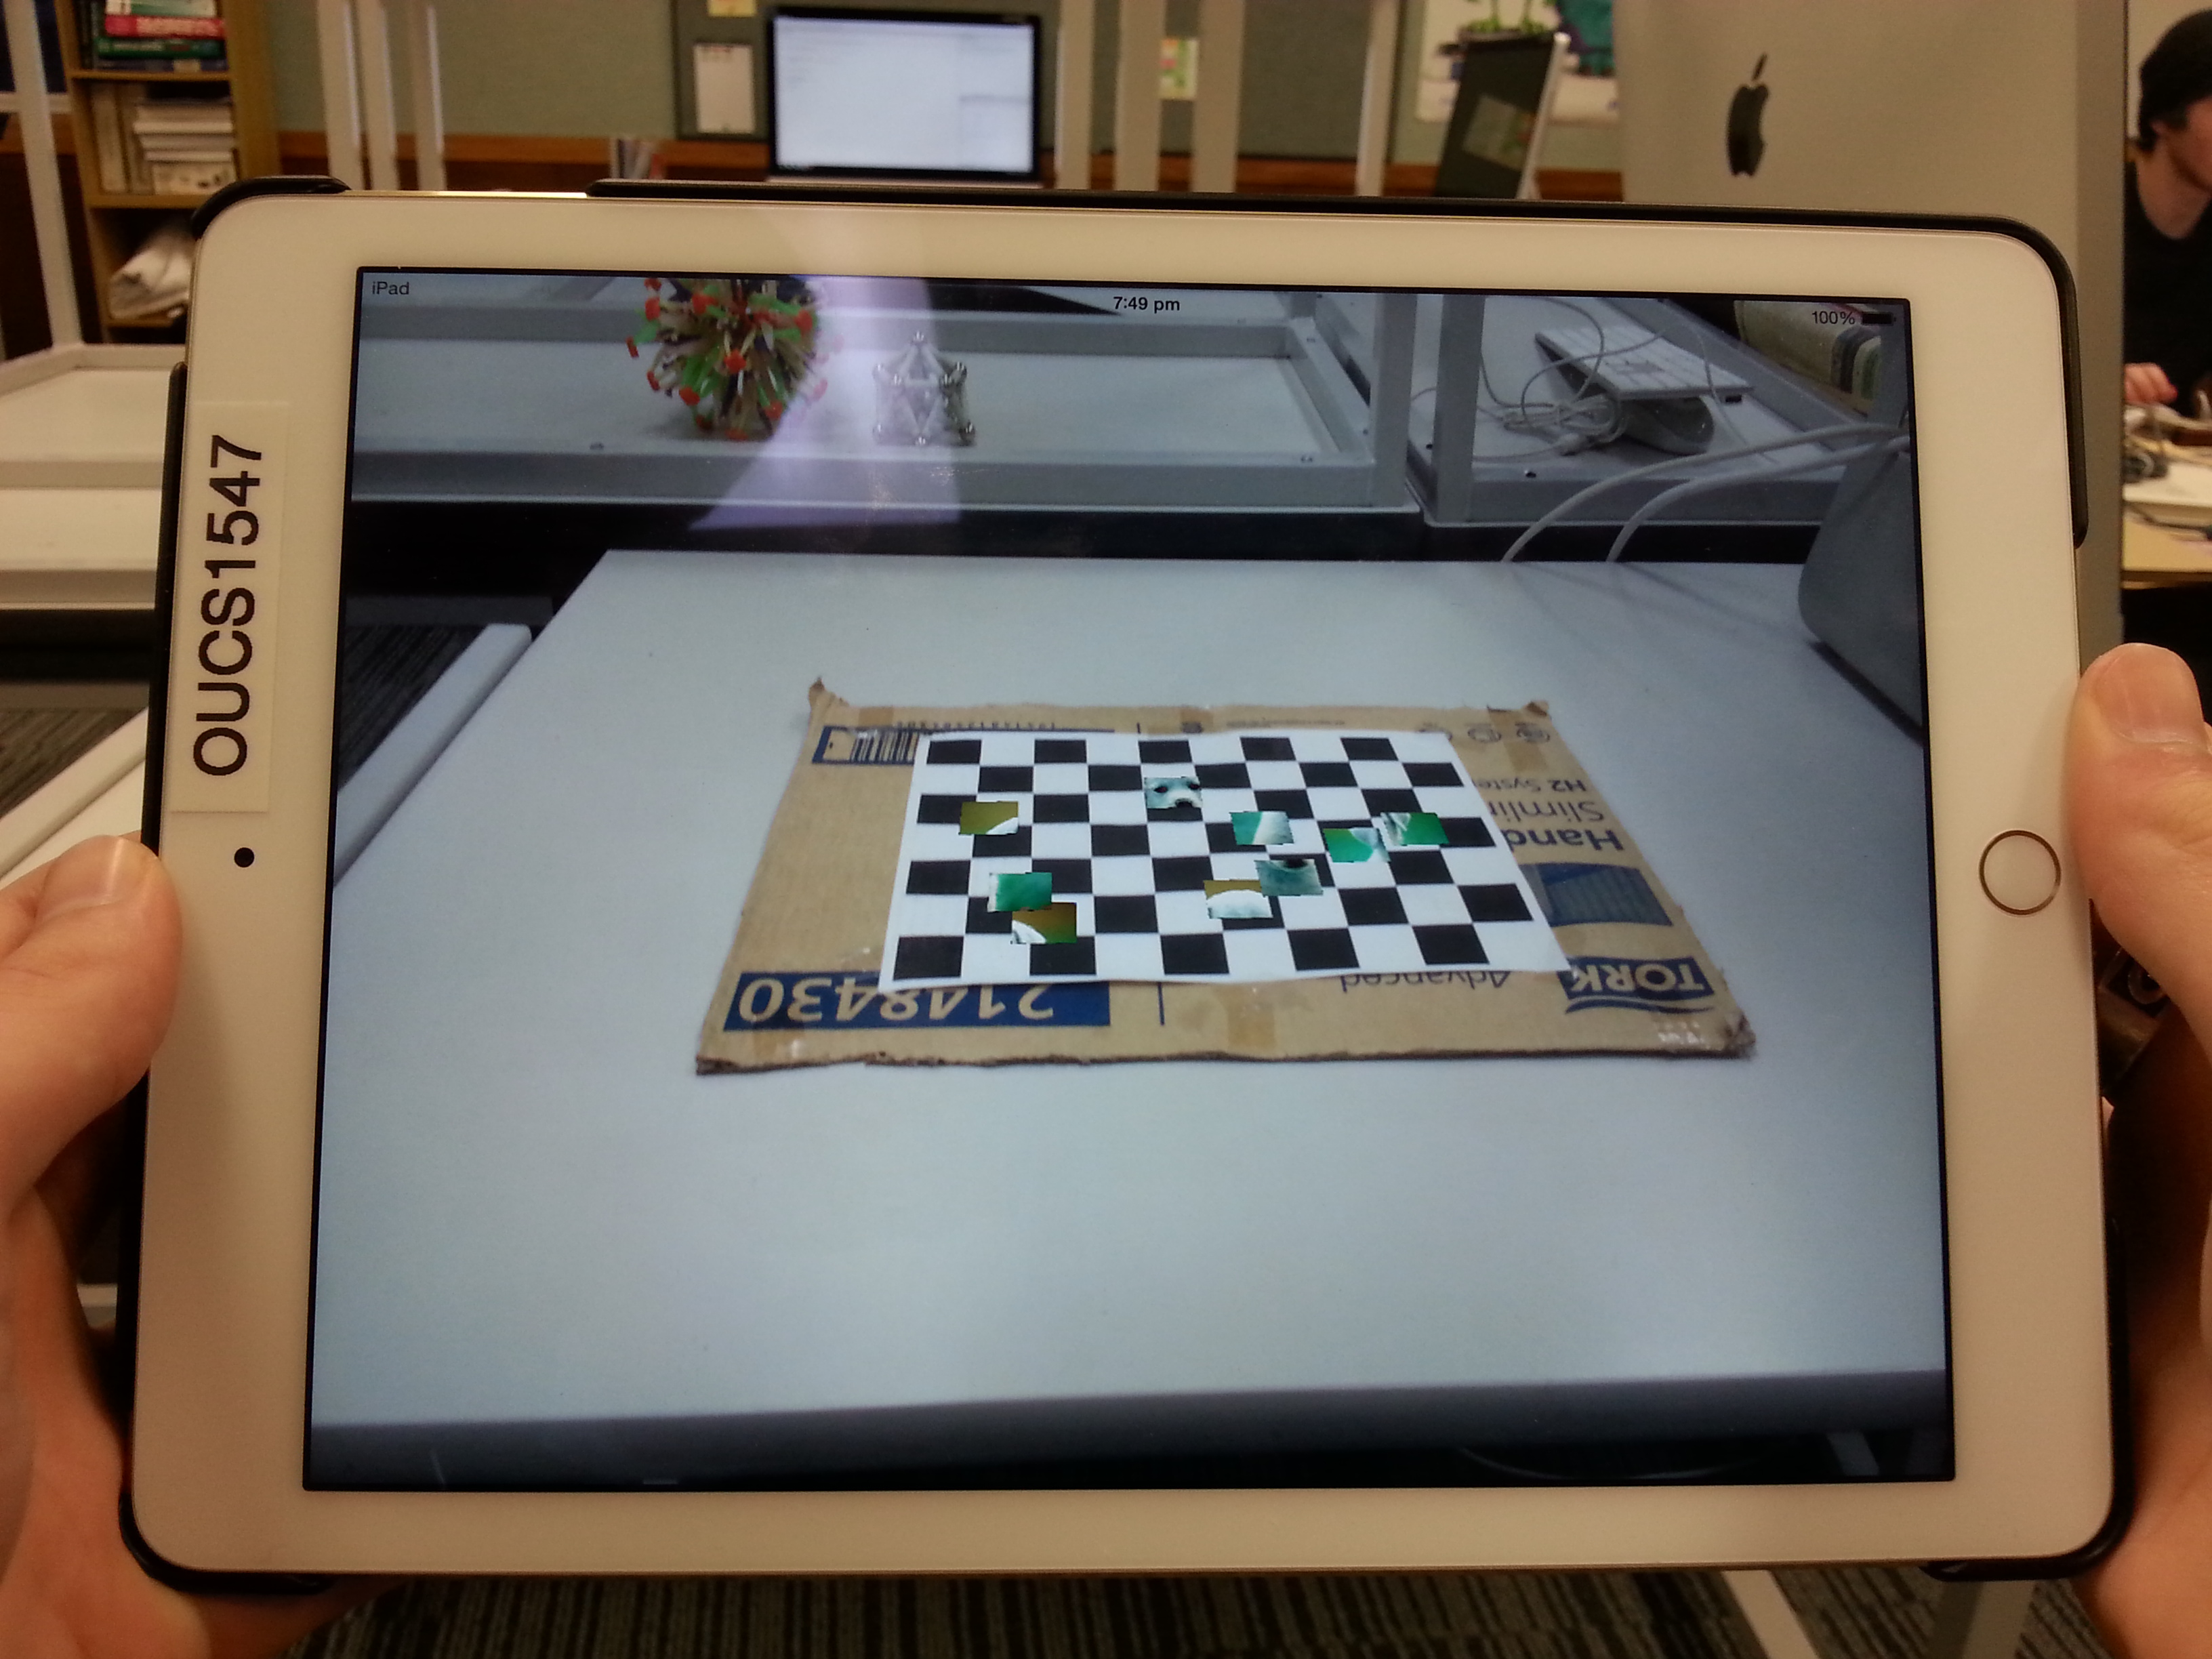
\includegraphics[width=0.49\textwidth]{low_angle}
\caption{Giguesaur running. Showing a high angle view and a low angle view. }
\end{center}
\end{figure}


\section{Discussion and Future Work}

\subsection{Localisation}
%Discuss those successes and failures and relate them back to aims and objectives. 
I didn't achieve everything that I had planned when I began work on the Giguesaur project. Initially my goal was to test a variety of different marker tracking techniques before choosing the best one and integrating it into the main application. In reality just getting some kind of marker tracking to work took much longer than expected. So rather than spend more time finding the optimal solution I decided to work with what I already had. This meant using the checkerboard pattern as a marker and OpenCV's function for locating its internal corners. 

When the project was much further along I discovered that the function for finding those corners is rather complex and takes approximately a fifth of a second to execute. This is the main reason that the application runs at around five frames per second. By this time it was far too late to change from OpenCV to some other marker tracking package so I decided to create my own marker tracking algorithm. I started programming a routine that would locate the centre of coloured blobs and return the coordinates. I would then use these coordinates as my image space points in the pose estimation algorithm. However I ran out of time and so the blob finder doesn't yet work with real camera input. Replacing the checkerboard finding function with a robust blob finder would likely improve the performance of Giguesaur significantly. This change would be the priority for future work on the application. 

Alternatively, the findChessboardCorners function could be speeded up by restricting the area of the image that it operates on. If you assume that the checkerboard pattern's position in the image is unlikely to change much from frame to frame then you could define a sub-image for the find checkerboard function to work on. That sub-image would be defined based on the position of the checkerboard in the previous frame. As the size of the sub-image is less than the size of the frame, it would take less time to process. This method would improve the frame rate of Giguesaur although probably not as much as the blob finder. If completion of the blob finder is not possible then the next best option would be to implement this method. 

My final objective for the Giguesuar project was to implement marker tracking that could handle the marker being obscured from view. Currently if the chessboard pattern has any of its internal corners covered the function that finds the corners won't return anything. There has been some research on the topic of partial marker occlusion \cite{occlusion} and I would have liked to be able to implement a similar system. Allowing for marker occlusion would make the application much more robust in a real environment so adapting Giguesaur to cope with this would be a marked improvement. 

If I were to start over on the Giguesaur project I think I would have chosen a different method for the marker tracking. OpenCV is a rather large library that is used for many different purposes and I think this diversity makes it less capable with specific tasks. If I had used a specially made marker tracking package such as the ARToolKit I think I might have achieved a more satisfactory result. 

\subsection{Game Logic and Interface}
Currently pieces are picked up and placed down only using taps on the iPad's screen. One of the initial goals of the Game Logic and Interface component of Giguesaur was to be able to rotate and position a held piece by positioning the iPad. The interface would show some kind of transparent piece locked to the screen with a shadow displayed on the board to represent where the piece would land when dropped. This goal wasn't reached due to time constraints. I think implementing this idea would make interacting with Giguesaur a more enjoyable experience.

The pieces of the Giguesaur puzzle are represented as simple quads. Another of the goals of the Game Logic and Interface component was to create pieces with curved edges, like a real jigsaw puzzle has. Having the pieces look more like real jigsaw pieces would be a significant visual improvment for Giguesaur.

\newpage
\section{Glossary}
 
\textbf{OpenGL}: A low level graphics API. Can be used to constuct complex graphics from geometric primitives.

\textbf{Preview Layer}: An Apple AVFoundation Framework object that takes input from an iOS device's camera and displays it to the screen.

\textbf{UIImage}: An Objective-C image format that is part of the Apple UIKit framework. Used by many functions within Apple's frameworks

\textbf{CMSampleBuffer}: The type of image buffer created by the PreviewLayer. The image data from the PreviewLayer gets stored as a CMSampleBuffer.


\section{Appendix}\label{appendix_sec}

The video mentioned in the results section along with a snapshot of all of the Giguesaur code can be found at the following link:

\textbf{https://github.com/ShahneRodgers/Giguesaur/releases}

\newpage
%----------------------------------------------------------------------------------------
%	BIBLIOGRAPHY - Check references. 
%----------------------------------------------------------------------------------------

\bibliographystyle{ieeetr}
\nocite{*}
\bibliography{references}

%----------------------------------------------------------------------------------------


\end{document}